\chapter{Background}

\section{Laser Trapped-Ion Experiment}

Trapped-ion quantum systems have emerged as a leading candidate for quantum computing platforms due to their exceptional coherence times, high-fidelity quantum gates, and promising scalability. In trapped-ion systems, ions—charged atoms confined by electric fields—are precisely controlled and manipulated using laser beams. These lasers serve critical roles, including initializing quantum states, implementing quantum gates, and performing state measurements [XX].

However, traditional approaches for optical hardware tend to be bulky, expensive, and power-intensive, posing severe limitations on scalability. As the number of qubits in a trapped-ion quantum computing system grows, these challenges become more pronounced [XX]. Compact, efficient, and rapid modulation capabilities are thus essential to scale quantum computing platforms beyond small-scale demonstrations.

Recent advancements in photonic integrated circuits (PICs) have substantially addressed these challenges [XX]. These PICs are miniaturized, enabling direct integration with ion-trap chips, thereby dramatically reducing optical losses, system complexity, and the overall footprint. Crucially, integrated modulators facilitate modulation at very high speeds—on the order of nanoseconds—which matches the stringent timing requirements of quantum operations [XX].

To fully utilize the capabilities of these advanced PICs, corresponding electronic control systems capable of generating precisely timed, flexible modulation signals at around 100 MHz resolution are necessary. The 100 MHz resolution provided by the system ensures that the modulation signals can be precisely timed and shaped, directly corresponding to the stringent timing requirements of quantum gates that often operate on microsecond timescales. Having 32 synchronous dynamic voltage channels is essential because it allows the simultaneous manipulation of multiple qubits with coherent precision, thereby supporting complex, parallel quantum operations [XX]. The precise synchronization of these channels ensures minimal timing jitter and improved gate fidelity, which is indispensable for scaling quantum computing systems to larger qubit arrays.

\section{Hardware Description}

To meet the demands of advanced control electronics, this project utilizes a Field Programmable Gate Array (FPGA). FPGAs excel at high-speed, low-latency parallel processing, enabling the simultaneous control of multiple channels and the implementation of flexible, efficient digital signal processing algorithms. These capabilities make FPGAs particularly suited for managing complex experimental setups that demand precise timing and real-time adaptability. For this project, we specifically employ the Xilinx Zynq UltraScale+ ZCU102 Evaluation Board, a robust platform chosen for its exceptional computational resources and flexible high-speed interfacing capabilities.

The ZCU102 board is integral for generating precise modulation signals required by quantum lasers. It features a range of peripherals, including PMOD interfaces that support low-speed digital-to-analog converters (DACs) via SPI protocols, and two FMC HPC connectors for high-speed DACs, essential for waveform generation. The core of this FPGA platform is the Xilinx Zynq architecture, which seamlessly combines a Processing System (PS) with Programmable Logic (PL).

The PS is powered by a quad-core Arm\textsuperscript{\textregistered} Cortex\textsuperscript{\textregistered}-A53 processor, capable of running real-time processing applications. It incorporates multiple peripherals, such as DDR4 memory for application storage and an Advanced eXtensible Interface (AXI) that connects the PS to other components, including the programmable logic. The PL, essentially the FPGA itself, is equipped with essential resources like logic cells, flip-flops, and 32.1 Mb of block RAM (BRAM), providing ample capacity for storing intermediate data.

This project leverages programmable logic to build custom hardware designs that serve the unique demands of quantum laser experiments. The FPGA's dedicated logic circuits and integrated high-speed interfaces enable quick, reliable communication with external modules. This capability is crucial for maintaining accurate control and precise timing—cornerstones for experiments where synchronization is everything. General-purpose I/O options, such as PMOD and FMC connectors, further simplify the experimental setup. These connectors offer flexible interfacing, allowing for both low-speed and high-speed connections that scale to the experiment's complexity without sacrificing performance.

In addition to the hardware features, a Python interface abstracts the low-level hardware details, streamlines testing and integration with the FPGA platform. Behind the scenes, a custom C-based program running in the processing system translates data from the Python interface into a format that the FPGA can efficiently process. This layered approach bridges high-level control with low-level hardware performance, ensuring that experimental algorithms and rapid prototyping can be achieved with reliability and precision.

\section{Pulse Sequence}

In high-fidelity quantum computing and atomic manipulation, pulsed sequences are essential for delivering precise, accurate, and stable outputs to photonic integrated circuits [XX]. These laser pulses depicted in \autoref{fig:pulse_seq} are designed with a controlled shape that consists of three distinct phases: rise, sustain, and fall. Each phase plays a vital role in ensuring that quantum operations are performed reliably.

\begin{figure}[h]
    \centering
    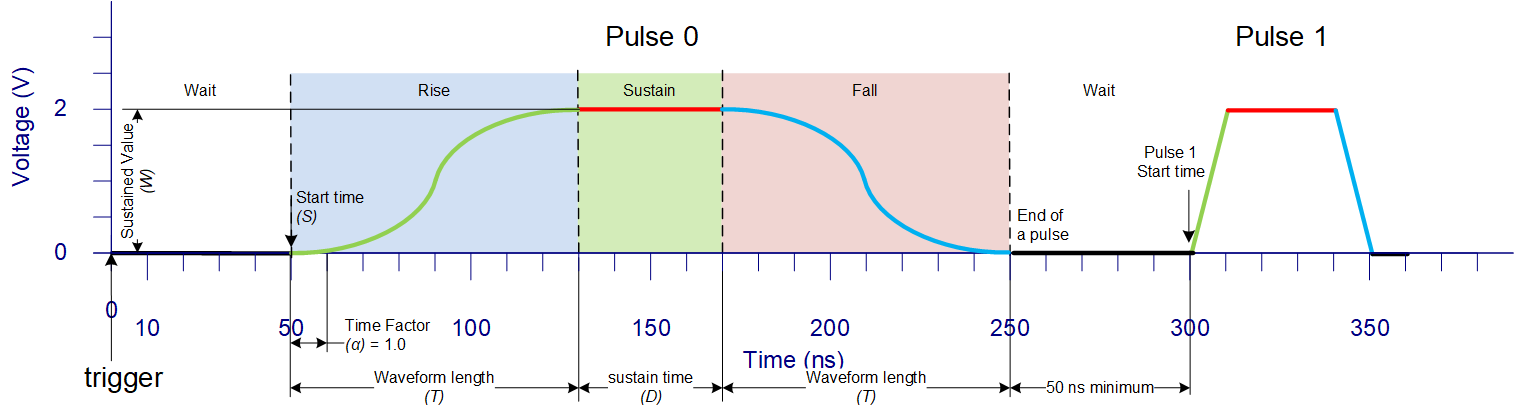
\includegraphics[width=1\linewidth]{figures/2.1.png}
    \caption{Waveform shape of the pulse sequence.}
    \label{fig:pulse_seq}
\end{figure}

During the rise phase, the laser intensity increases to its target level. The speed of this increase governs the timing of quantum gate operations. A well-controlled rise minimizes phase errors and ensures that the gates operate exactly when needed [XX]. The sustain phase follows, during which the laser maintains a constant optical intensity. This steady state is crucial because any fluctuation can compromise the fidelity of quantum gates by introducing operational errors. Finally, the fall phase allows the laser power to decrease smoothly. A controlled fall minimizes unintended transitions and residual effects, which could otherwise disturb the delicate quantum states. Notably, maintaining symmetry between the rise and fall phases is critical for consistency and repeatability. In this design, the fall essentially becomes the reciprocal of the rise.

From a hardware perspective, the waveform is generated as a series of discrete values representing a continuous function, with samples taken every 10 nanoseconds by the digital-to-analog converter (DAC). These sample values can be adjusted to fine-tune the laser's output. For a waveform $f(x)$, a pulse generated by the hardware to the laser can be defined by:

\begin{equation}
g(x) = A \cdot 
\begin{cases} 
f\left(\dfrac{\alpha(x - S)}{T}\right), & \!\!\! S \leq x < S + \left\lceil \frac{T-1}{\alpha} \right\rceil, \\[8pt]
f\left(\dfrac{T-1}{T}\right), & \!\!\! S + \left\lceil \frac{T-1}{\alpha} \right\rceil \leq x < S + \left\lceil \frac{T-1}{\alpha} \right\rceil + D, \\[8pt]
f\left(\dfrac{\alpha\left(2\left\lceil \frac{T-1}{\alpha} \right\rceil + D - (x - S) - 1\right)}{T}\right), & \!\!\! S + \left\lceil \frac{T-1}{\alpha} \right\rceil + D \leq x < S + 2\left\lceil \frac{T-1}{\alpha} \right\rceil + D - 1, \\[8pt]
0, & \!\!\! \text{otherwise}.
\end{cases}
\end{equation}



Where $S$ is the pulse start time, $T$ is the waveform rise's length, $\alpha$ is the time factor, $D$ is the sustain time, and $A$ is the gain factor.